%!TEX root = ../thesis.tex

\chapter{Implementierung} % (fold)
\label{cha:implementierung}


\begin{itemize}
    \item Probleme und deren Lösung während der Umsetzung
    \item Beispiel: Zugriff auf Moodle über Webservice
\end{itemize}

\begin{figure}[ht]
     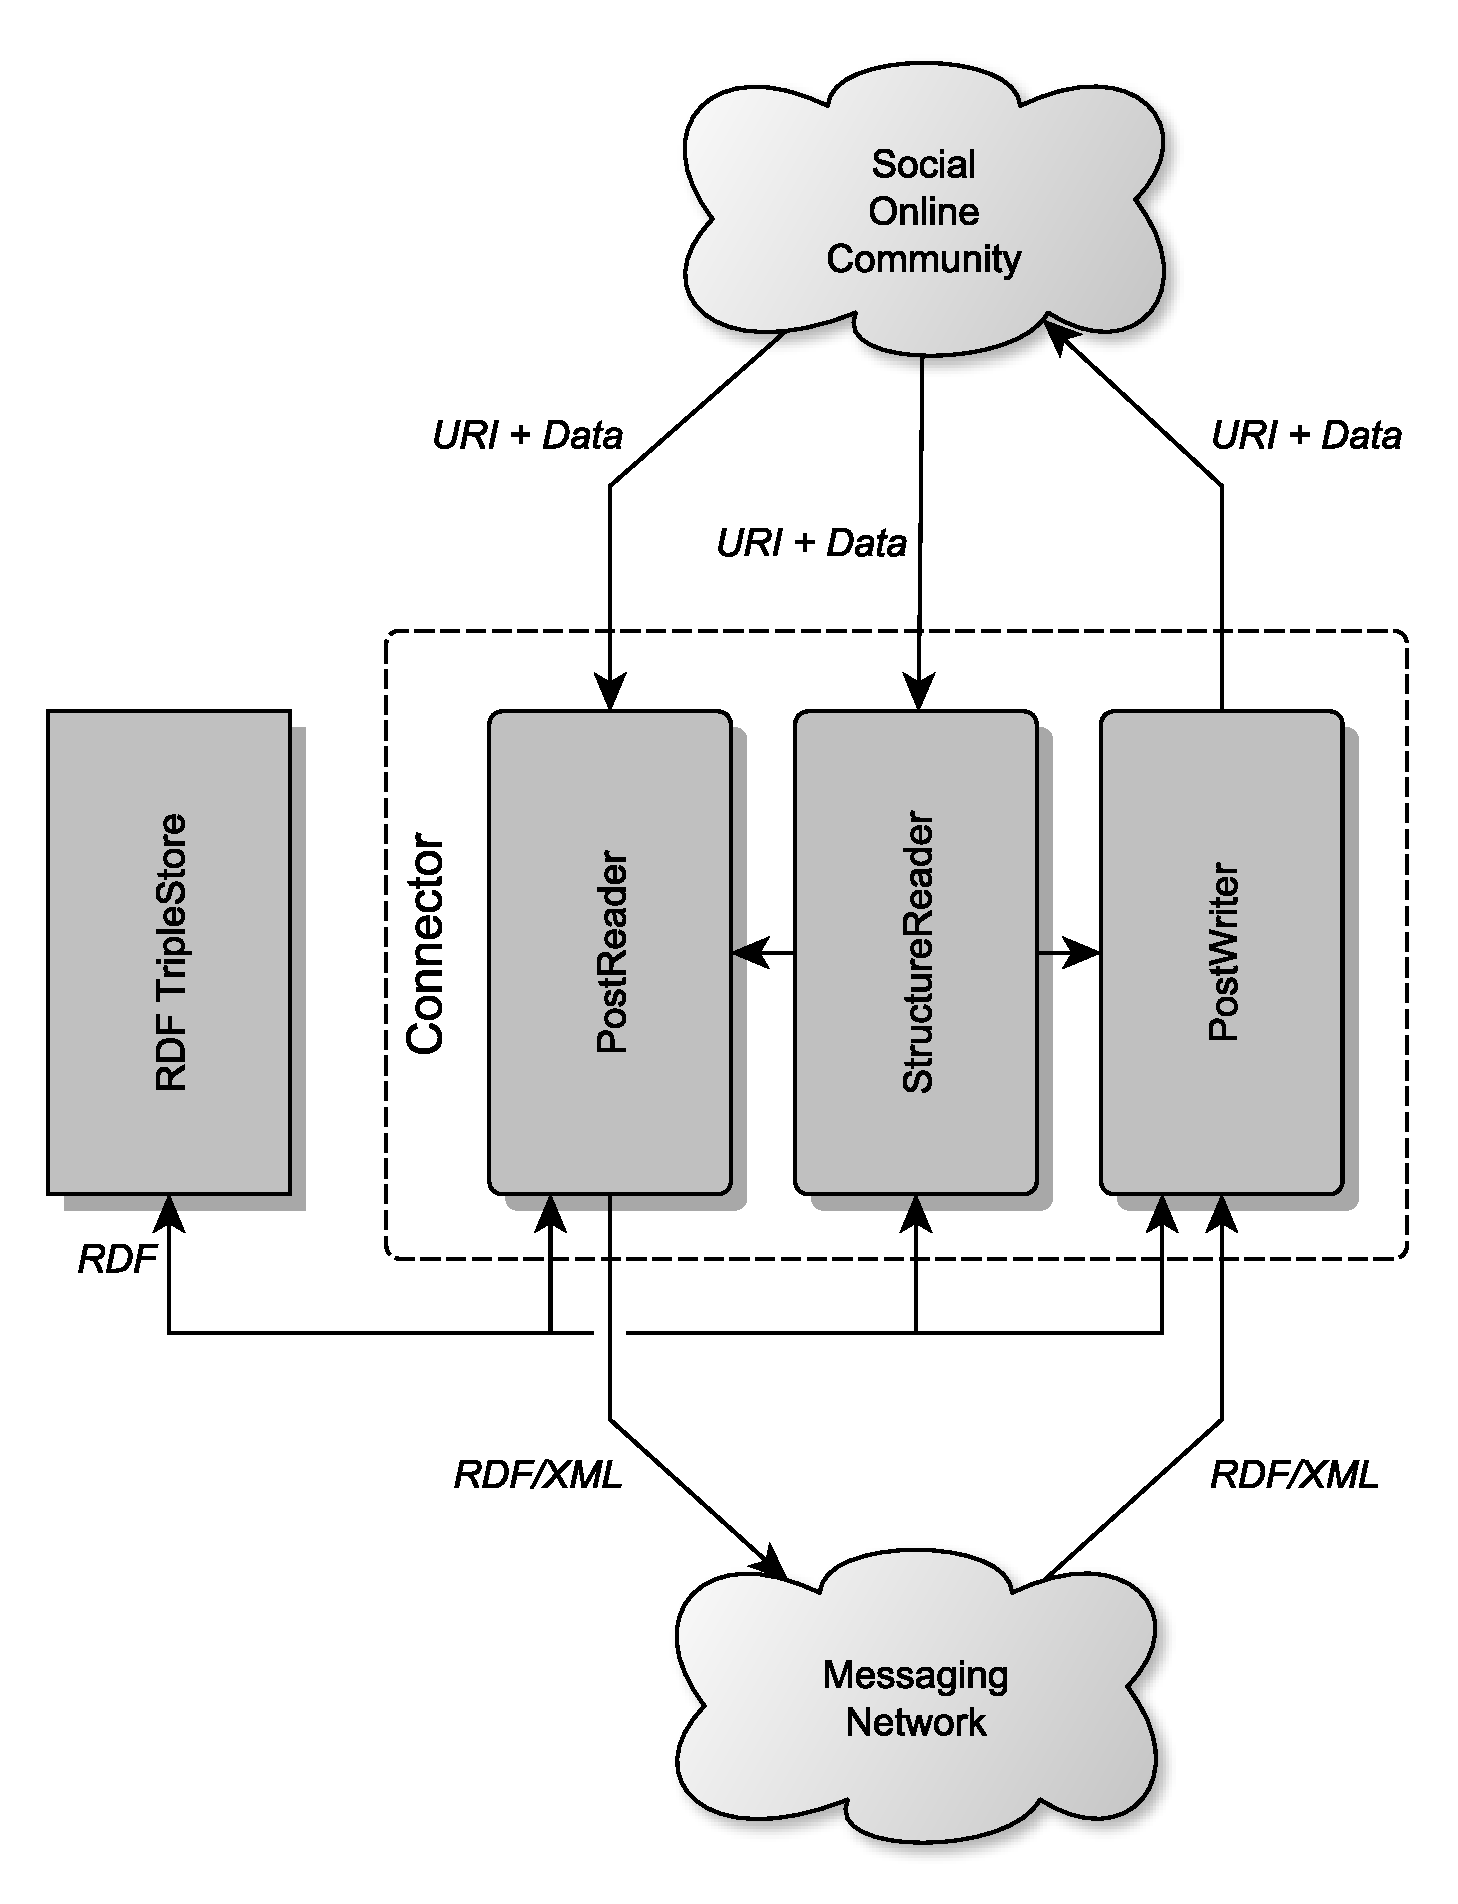
\includegraphics[
        width=\textwidth,
        keepaspectratio=true
    ]{assets/images/socc_connector_overview.pdf}
    \caption{Übersicht der Komponenten der SOCC}
    \label{fig:uebersicht_socc}
\end{figure}

\begin{figure}[ht]
     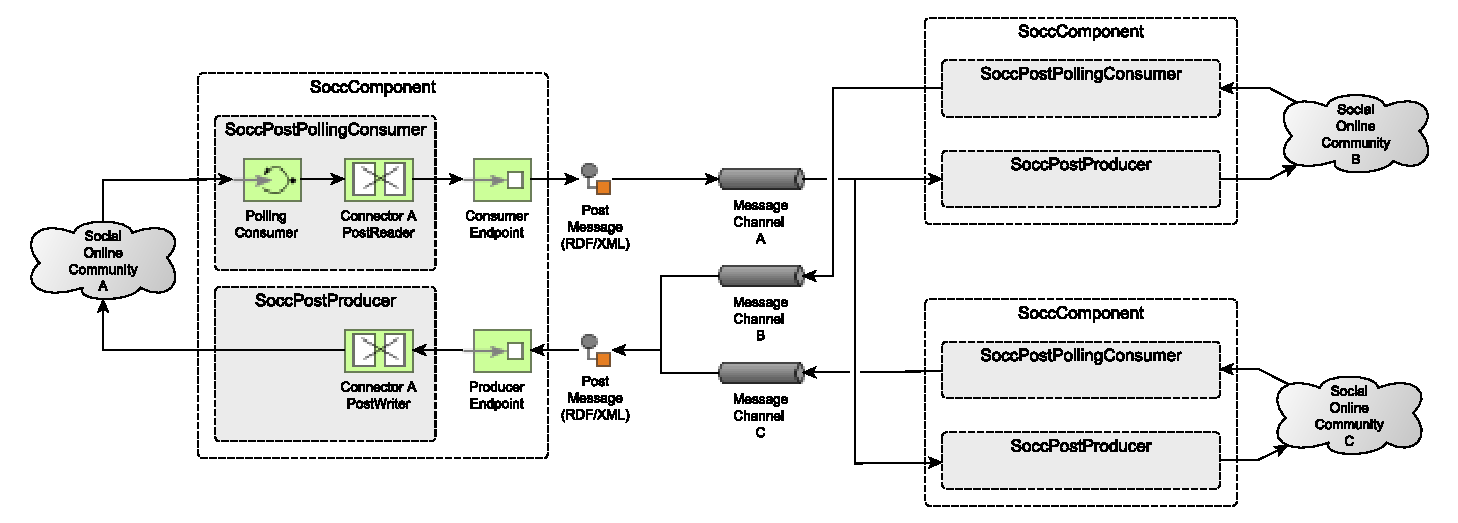
\includegraphics[
        width=\textwidth,
        keepaspectratio=true
    ]{assets/images/socc_camel_overview}
    \caption{Übersicht des Apache Camel Moduls Socc-Camel}
    \label{fig:uebersicht_socc_camel}
\end{figure}


%------------------------------------------------------------------------------

\section{Verwalten SIOC Daten} % (fold)
\label{sec:zugriff_auf_sioc_daten}

\begin{itemize}
    \item Sesame, Jena -> RDF2Go
    \item In Memory, XML/RDF File, Tripplestore 
\end{itemize}

%------------------------------------------------------------------------------

\section{Zugriff auf Online Netzwerke und Abbildung in SIOC} % (fold)
\label{sec:zugriff_auf_online_netzwerke_und_abbildung_in_sioc}

\subsection{Moodle} % (fold)
\label{sub:moodle}

\subsection{Canvas LMS} % (fold)
\label{sub:canvas_lms}

\subsection{Facebook} % (fold)
\label{sub:facebook}

\subsection{Google Plus} % (fold)
\label{sub:google_plus}

\subsection{Youtupe} % (fold)
\label{sub:youtupe}

%------------------------------------------------------------------------------


\section{Implementieren der Connectoren} % (fold)
\label{sec:implementieren_der_connectoren}

\begin{itemize}
    \item 
\end{itemize}

% chapter implementierung (end)
